\chapter{Introduction} \label{ch:introduction}
%  - clouds, climate and machine learning
Clouds play a\textcolor{red}{n} important role in the climate system. Both affecting the radiative budget and the hydrological cycle. \textit{Consist/Composed of liquid droplets, ice crystal or both.} Understanding how clouds form in the complex system of the atmosphere involves both \textcolor{red}{(Both brukes nå rette etter hverandre i to setninger dersom du ikke skal ha med den i kursiv. Kanskje du bare kan droppe "both" i denne setningen?)} knowledge about the large scale influence by the circulation and the small scale influenced by aerosols. To this day the micro-physics of all phases are not fully understood. Here mixed phase clouds, clouds consisting of both liquid and ice, \textit{proofs}(\textcolor{red}{(Kan du bruke noe så enkelt som "shows"?} to be the most difficult. 
\\ \\ 
Climate models are the most useful tool for studying \textcolor{red}{the?} past, present and future climate change. Clouds and aerosols are acknowledged as the factor\textcolor{red}{s} contributing with the largest uncertainty to the \acrfull{ecs}. Also know\textcolor{red}{n} as global mean temperature increase due \textcolor{red}{(Kan også bruke "as a consequence" istedenfor due hvis du ender opp med å bruke mye "due to")} to a doubling of the pre-industrial levels of $CO_2$ (280 \acrshort{ppm}). \textcolor{red}{Burde ha en kildehenvisning her} \textit{It remains unclear to which level of sophistication is adaquate to model their effect om climate.} \textbf{Siter ch7 AR5}. 
\\ \\
\textbf{Make sure you include everything that's related to parametrized processes.} It is understood that cloud formation requires suitable aerosol\textcolor{red}{s} and sufficient supersaturation. Aerosols include both gases and solid particles suspended in air. They interact with the clouds by serving as particles which vapour and ice can condensate or deposit upon. The different phases require different properties and the nuclei's \textcolor{red}{Er det bare "nuclei"? Nuclei skulle være pluralformen til ordet nucleus, så vet ikke om det blir dobbelt opp med flertall med den s-en bak.Men hør med noen bedre språkeksperter enn meg} are called \acrshort{ccn} for liquid droplets and \acrshort{inp} for ice crystals. Saturation is usually archived by a temperature decrease in rising air masses. Thus the stability of the atmosphere affect \textcolor{red}{fjerne affect?} plays a key role for convective motions. \textbf{What drives convective motions? Temperature differences.}
\textbf{Legg inn bilde a skyer en i is fase og en i liquids. Skriv noe som "the sharp outoline suggest that the cloud is consisting of liquid droplets, even at temperagtures below 0."}
%The negative temperature decreases by height is often referred to as the lapse rate, $\Gamma_{s, d}$. 
\\ \\ 
Growth processes are phase dependant. Liquid droplet grow\textcolor{red}{s} by diffusion and later by collision and coalescence. At temperatures -38/-40 degrees \textcolor{red}{C?} \textbf{kilde} they will spontaneously freeze and could play the role as \acrshort{inp}. When both phases are present in a cloud, the saturation vapour pressure over ice is higher than over liquid. This may cause the droplets to evaporated and depositing on to the ice crystals  \textcolor{red}{(I denne setningen skriver du i to tider. Hva med å bytte evaporated med evaporate og depositing med deposit)}. This is called the Wegeron-Bergeron-Findeisen process. Clouds consisting sole  \textcolor{red}{(Høres litt rart ut og etter å ha søkt litt i cambridge sin ordbok virker det som at de bruker ordet på en litt annen måte enn det som fremkommer her, men kan selvfølgelig hende at jeg tar feil. Det er mulig å bruke "solely", men tror "sole" alene blir litt feil. SOm sagt, ingen ekspert. Mulig å bruke "purely", "singly", "only" eller "soley" tror jeg høres bedre ut )} of ice crystals first grow by deposition of vapour then by aggregation. 
\\ \\ 
Due  \textcolor{red}{( 1) Prøv å ikke start setningen med "due to". Jeg synes "Because of" i så fall høres bedre ut, men vegard synes ikke nødvendigvis "because of" høres bedre ut. 2) Dette er ikke en ordentlig setning. Må i så fall fjerne punktum og sette et komma. Kommer tilbake med forslag her... Mulig å si noe sånt som \textit{Lots of different processes occurring simultaneously on different scales due to the complex nature of clouds.} )} to the complex nature of clouds. Lots of different processes occurring simultaneously on different scales. Incorporating all these interactions into a model framework has proven to be difficult\textcolor{red}{(Her må du ha en kilde og gjerne flere siden du hevder noe er vanskelig å bevise)}. \textbf{Read ch. 2 at Statkraft i helga.} Explain convection and fronts. Mention cumulus, status and cirrus clouds?
Include observational changes in the hydrological balance. 

\section{Clouds in the current climate} \label{sec:intro_cloud_current_climate}
\begin{figure}[h] % small h, setter den rett under teksten.
    \centering
    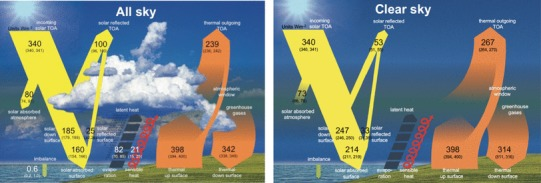
\includegraphics[scale = 7]{Chapter1_Intro/images/both_wild2019.jpg}
    \caption{The all-sky and the clear sky. Figure 14 Wild 2019. Ikke i bruk vennligst kommenter om denne er bedre enn den andre som viser differences mellom disse subplottene.}
    \label{fig:both_wild}
\end{figure}

Based on satellite and ground based measurements Wild et. al. 2019 \textbf{siter} have quantified the contribution of elements in the radiative budget. Subtracting the clear-sky from the all-sky climatology to compute the \acrfull{cre}. This is shown in equations \eqref{eq:cre_sw} and (\ref{eq:cre_lw}). Wild et. al. 2019 \textbf{siter} concludes with a reduction in shortwave radiation of $-47Wm^{-2}$ by clouds. In other words clouds reflect approximately 50\% of the incoming solar radiation. Longwave component is $28Wm^{-2}$. This give a net \acrshort{cre} of $-19Wm^{-2}$. Proving that the net effects of clouds on the radiative budget is negative.The altitude along with the composition determines the radiative properties of the cloud. \textbf{Relate this to the black body properties of clouds..? LES Artikkel fra Jonah}
\begin{figure}[h]
    \centering
    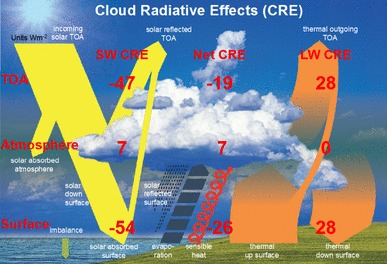
\includegraphics[scale = 7]{Chapter1_Intro/images/CRE_wild2019.jpg}
    \caption{Cloud radiative effect, CRE is the differece between the radiative components of the Clear sky radiative and the all sky. Cite this figure as fig 15 in Wild 2019}
    \label{fig:cre}
\end{figure}

\begin{equation} \label{eq:cre_sw}
    CRE_{sw} = SW\uparrow_{clear-sky} - SW\uparrow_{all-sky}
\end{equation}
\begin{equation} \label{eq:cre_lw}
    CRE_{lw} = LW\uparrow_{clear-sky} - LW\uparrow_{all-sky}
\end{equation}
\\
The physical properties causing the interaction with radiation is described below. Dense low level clouds reflect solar radiation. This is called the albedo effect. Albedo (\textcolor{red}{(Jeg fikk beskjed av en av mine veiledere at alle ting man forklarer som f.eks. albedo må stå i kursiv, men det skal sies at han "bare" hadde en doktorgrad og var litt old school, men du kan jo se litt hva andre har gjort)} being the ratio between reflected to incoming radiation. The higher number \textcolor{red}{of?} concentrations of droplets in a cloud the higher the total surface area of droplets. The more radiation gets reflected back into space \textcolor{red}{(Ikke en fullstendig setning slik jeg ser det. Kan fungere med et komma, men den blir kanskje veldig lang. Kan fungere med "The size/extent of the surface area of droplets affects the amount of radiation reflected back into space." eller "Large surface area of droplets reflects more radiation back into space}. Clouds absorb longwave radiation and re-emits it. The absorbed radiation originates from the surface and is given by Stefan-Boltzmann forth-power law, see equation (\ref{eq:stefan-boltzmann}). \textbf{En setning om at jordkloden er mye mer like en black body enn det is, vann og snø krystsller er. Selv om de også emitter som en funksjon av temp. } High clouds have low temperatures and since the re-emitted flux is a function of the cloud temperature. The greenhouse effect increases with the height of the clouds.

\textcolor{red}{Jeg likte den første figuren best. Synes forøvrig at begge har liten tekst og det er vanskelig å lese hva som står under fluksene. Kanskje mulig å lage en bildetekst under det første som presiserer at det er differansen mellom bildene og si at 100-53 er 47 eller noe. Husk at bildeteksten skal kunne stå for seg selv uten at leseren leser oppgaven}




\begin{equation} \label{eq:stefan-boltzmann}
    F = \sigma T ^4
\end{equation}

\section{Clouds in future climates} \label{sec:intro_cloud_future_climates}
\begin{figure}[h]
    \centering
    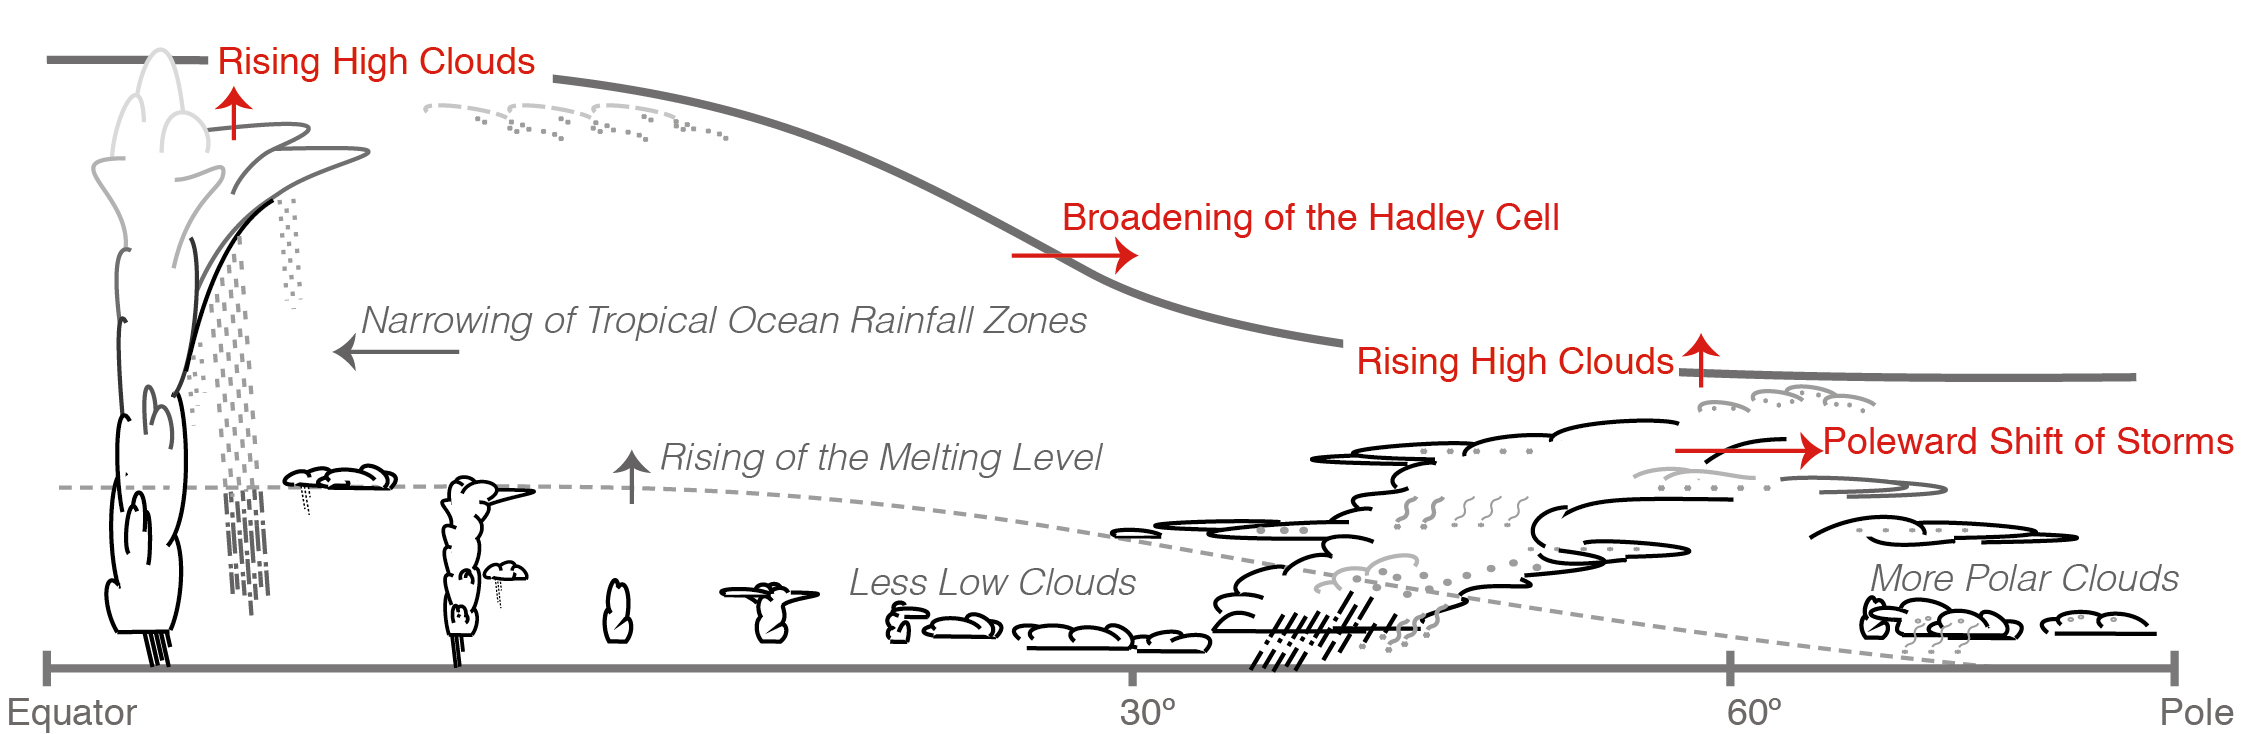
\includegraphics[scale = 0.8]{Chapter1_Intro/images/Fig7-11_ipcc.jpg}
    \caption{Cloud climatology in future climate. Developed based feedbacks in climate models, the different adjustments have different sikkerhet. Cite the fifth assessment report IPCC report.}
    \label{fig:cloud_scheme}
\end{figure}

Wild et. al. 2019  \textbf{siter} finds a\textcolor{red}{n} imbalance of $0.6W m^{-2}$ \textcolor{red}{(Ubalanse hvor da? HEr mangler det litt forklaring.Kanskje du kan nevne dette litt lenger ned og heller skrive " Excess of radiation gets trapped in the earth system, forcing the surface temperature to increase in order to close the radiative budget." Vet ikke om det blir helt riktig, men tenker du må ha en annen start eller bedre overgang fra forrige avsnitt )}. This heat gets trapped in the earth system, forcing the surface temperature to increase in order to close the radiative budget. The imbalance in the radiative budget at \acrshort{toa} \textcolor{red}{Du har ikke forklart hva TOA er eller brukt det fulle navnet. Du må alltid bruke det fulle navnet første gang du snakker om det} is the radiative forcing. Climate drivers include both natural and ant\textcolor{red}{h}ropogenic forcings. This can be everything from natural variability in the solar energy output, v\textcolor{red}{o}lcanic eruptions and green house \textcolor{red}{(vær konsekvent. I forrige avsnitt så skrev du "greenhouse" og nå skriver du "green house")} gas emis\textcolor{red}{s}ions. The overall goal is to compute the climate sensitivity/equilibrium temperature as a function of forcing \textcolor{red}{(Er dette ditt mål? Er det klimamodellerere? Hvis det er din problemstilling burde det komme bedre frem)}. For different \acrfull{rcp} scenarios one get a different temperature increase \textcolor{red}{(Denne setningen skjønte jeg ikke helt. Prøv også å ikke bruk "/". Bestem deg for enten "sensitivity " eller "equilibrium")}.
\\ \\ 
The global temperature will keep rising until we \textcolor{red}{(Ikke bruk "we", "I", "us", etc. skriv i såfall "it")} have reached the equilibrium climate temperature. This temperature increase induces climate changes. The \acrshort{ipcc} \textcolor{red}{(Heller ikke forklart IPCC med fullt navn i teksten før. Er ganske annerkjent, men må fortsatt forklares i full tekst første gang)} suggest\textcolor{red}{s? (Er IPCC flertall eller entall? Trodde det var entall, men litt usikker her)} the following shift in cloud schemes (see figure \ref{fig:cloud_scheme}). A broadening of the Hadley cell causes a poleward shift of storms. \textbf{spinn bevart lenger nord?} The albedo effect decrease\textcolor{red}{s} at higher latitude. Moving the dense clouds further into the polar night. %Only the greenhouse effect of theses clouds persist. 
The greenhouse effect of clouds still persist without sunlight leading to a net heating in the Arctic. Rising higher clouds causing a stronger greenhouse effect of clouds.
\\ \\
Aerosols can alter the cloud micro-physics and in terms alter the radiative properties of the cloud. A polluted cloud gets extra \acrshort{ccn}, this results \textcolor{red}{(Kan du bytte ut "this results" til "resulting")} in more \textcolor{red}{(Rart å skulle si "more smaller"? Er ikke det litt smør på flesk som lyder feil?} smaller droplets, as they share the available liquid. This increases the total surface area of the droplets. Which \textcolor{red}{(Hvis det er et spørsmål kan du starte med "which", men dette blir bare en leddsetning når den står slik)} again reflect more radiation and could led to a enhanced lifetime, since it takes longer for the droplets to reach precipitation size \textcolor{red}{(This increases the total surface area of the droplets. It takes longer time for the droplets to reach precipiation size because an increase of reflected radiation could le\textcolor{red}{a}d to a enhanced lifetime.)}. If it does, it might not since only one out of ten cloud precipitate \textcolor{red}{Denne var litt rar, her må du lese gjennom på nytt og omformulerer. Her er et dårlig forslag, men likevel et forslag "If it reach precipitation size, it might not become/reaches a cloud that percipitate since only one out of ten clouds percipitate" Her må du også ha kilde når du kommer med sånne tall/statistikk}. \textbf{cloud physics book} When clouds persipitate they clean the air by removing particles.
\\ \\ 
Narrowing of the Tropical ocean rainfall zones \textcolor{red}{(Heter sonen "Tropical ocean rainfall zone" eller er det en regnsone over "Tropical ocean"? Hvis det er sistnevnte ville jeg foreslått "Narrowing of the rainfall zone above the tropical ocean...")} causes a drier subtropics. Rising of the meltlayer can cause the ice crystals to melt. This will results in more opaque clouds. \textcolor{red}{(Mulig å slå sammen setningen, men vet ikke om det blir bedre eller ikke. " Rising of the meltlayer can cause the ice crystals to melt, resulting in more opaque clouds". Da må du kanskje også starte neste setninge med "These opaque clouds...".)} These have a higher albedo and reflect more sunlight. \textbf{read page 591-592 again.}
\\ \\
Cloud micro-physical processes are not yet fully understood \textcolor{red}{(Kilde?)}. Along \textcolor{red}{(Synes "along" høres litt rart ut, men det er kanskje også fordi jeg ikke helt skjønner forbindelsen med forrige setning. Ønsker du å si at at det heller ikke er forstått i modellene? } with the fact that clouds are formed a\textcolor{red}{t(?)} smaller scale then can be resolved in your \textcolor{red}{("your"? Bedre med "the"?)} average climate models. Paramet\textcolor{red}{e}rization \textcolor{red}{(Siden du skriver de fleste ordene på britisk ville jeg brukt "parameterisation" (https://wikidiff.com/parameterize/parametrize))} are used to include the contribution from the subgrid scale processes to the mesoscale proces\textcolor{red}{s}es (weather phenomenons) in climate models and in weather predictions in general. Over the last years this has gained more attention since its acknowle\textcolor{red}{d}ged as the largest contributor to the uncertainty in climate models \textcolor{red}{(Her må du ha kilde)}. I'll \textcolor{red}{(Ikke bruk jeg, med mindre du har snakket og blitt enig med veilederen din om at du skal gjøre det. Hvis du ikke skal bruke jeg-form foreslår jeg "This topic is described in further detail in chapter \ref{ch:theoretical_back}" eller "Further details about the topic/uncertainty from parameterisation of clouds in climate models is described in chapter \ref{ch:theoretical_back}")} get back to this in chapter \ref{ch:theoretical_back}.

\section{Deep Learning} \label{sec:intro_deep_learning}
Artificial intelligence \textcolor{red}{(AI)} dates back to the fifties when pioneers start talking about \textit{automating task normally performed by humans} \textcolor{red}{(Hvis det du har i kursiv er et sitat så MÅ du ha kilde, eller så må du omskrive det)}. Machine learning is a means to achieve artificial intelligence. The progress in the field follows a sigmoid curve. Slow increase at first, then really steep, before it slows down again (see figure \textbf{ref sigmoid activation func}). Over the years there have been several discoveries kick-starting the development in machine learning. The very first algorithm's \textcolor{red}{(Tror det skal være "algorithms" og ikke "algorithm's")} include probabilistic modelling. Using the principles of statistics to analyse data \textcolor{red}{(Tror jeg ville kombinert de to setningene "The very first algorithms include probabilistic modelling, sing the principles of statistics to analyse data"}. This includes Naive Bayes classifiers and logistic regression. Two algorithm's \textcolor{red}{Tror også her at det er "algorithms" siden du snakker om flertall, algoritmer, og ikke algoritmens egenskaper.} which predates computers and are still useful today. Three main bottlenecks of advances in AI is \textcolor{red}{(are?)} hardware, data and algorithm's. Internet continuous to provide large amounts of data from Wikipedia, Flicker (tagged images) and YouTube. Advances in computational powers, such as graphical processing units, GPU's \textit{provide a environment/platform to learn in/on}. These where originally develop\textcolor{red}{ed} for the gaming industry, but in 2007 they realised a interface called CUDA (2007) which allows for computing \textbf{find a up to date cost and flops (floating point operations per second)}. \textbf{siter Chollet bok}
\\ \\ 
For clarity, the deep in deep learning refer\textcolor{red}{s} to the number of layers. Moving from shallow networks to deeper ones (more than 10)\textcolor{red}{, (?)} algorithmic advances in gradient propagation was needed. This includes activation functions, weight initialisation and optimisation schemes. I'll get back to that in section \ref{sec:intro_machine_learning} \textcolor{red}{(Igjen, er det greit for veileder at du skriver i jeg-form?)}. Other advances like batch normalisation, depth wise separable convolutions attributed to the revolution of \acrshort{ai}. 
\begin{figure}[h]
    \centering
    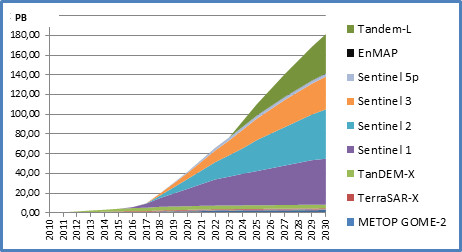
\includegraphics{Chapter1_Intro/images/Datenvolumen_D-SDA.jpg}
    \caption{Data volume. By the continuous earth system monitoring, meteorology/ climate science have progressed toward becoming a big data science. Observations are most used for verifying climate models and quantifying the current state of climate. \href{https://www.dlr.de/eoc/en/desktopdefault.aspx/tabid-12632/22039_read-51751}{https://www.dlr.de/eoc/en/desktopdefault.aspx/tabid-12632/22039{\_}read-51751}.}
    \label{fig:data_volum_sat}
\end{figure}
Earth system monitoring provides a global view of variables across meteorological systems. \textbf{Some thing about satellite era}. These large amounts of data and the flexible nature of the neural network makes is \textcolor{red}{it (?)} a suitable method also in geosciences. \textbf{With enough data neural networks can serve as a universal function approximate given a suitable hyper parameter tuning and input data.} The last couple of years reaserchers \textcolor{red}{(researchers?)} have been attempting to use this for wide range of problems like rainfall runoff model\textcolor{red}{l(På amerikansk er det 1 l, mens på britisk er det 2 l-er og du har valgt å bruke de britiske måtene å skrive på tidligere så ville holdt meg til det)}ing (krazerts), high-resolution weather forecasting (Rodrigues), Air quality forecasting (sun and liu), precipitaiton nowcast\textcolor{red}{i(?)}ng (Shi et al) and \textbf{kanskje: LES} \textit{deep neural network based feature representation for weather data.} \textbf{lui et al }. \textbf{noe med forskjellig hell.} Another more comprehensive machine learning project is lead by Tapio Schneider at Caltech. Along with his team og \textcolor{red}{and (fjern "og")} technologist\textcolor{red}{,} they have ambitions to create a earth system model using machine learning \textcolor{red}{Kanskje heller skrive, "Schneider, his team and technologist have ambitions..."}. With his team of from MIT and former employees of Microsoft and Google \textcolor{red}{Kanskje "The team consist of former employees from Microsoft and Google"? Men er det egentlig viktig å vite hvor teamet hans er fra? }they hope to create a platform which can resolve clouds and hopefully reduce the spread in climate sensitivity \textcolor{red}{in climate predictions (?)}. \textbf{cite science}

\textcolor{red}{Tenker at du har en veldig lang introduksjon hvor jeg ikke vet helt hvor du vil. Ja du forklarer masse greier og det kan man i en innledning, men da må man innledningsvis gi en kort introduksjon og presentere problemstillingen før man går over på tidligere arbeid og kanskje litt mer detaljert rundt maskinlæring, skyer og alt det bra du har skrevet i denne delen Det er mine tanker da. Og selv på slutten av introduksjonen nå så vet jeg fortsatt ikke hva du prøver å finne ut av, annet enn at du har forklart meg litt om skyer og maskinlæring så jeg kan anta at det er det du skal holde på med. }
